\documentclass[letterpaper,10pt,titlepage]{article}

\usepackage{graphicx}                                        
\usepackage{amssymb}                                         
\usepackage{amsmath}                                         
\usepackage{amsthm}                                          

\usepackage{alltt}                                           
\usepackage{float}
\usepackage{color}
\usepackage{url}

\usepackage{balance}
\usepackage[TABBOTCAP, tight]{subfigure}
\usepackage{enumitem}
\usepackage{pstricks, pst-node}

\usepackage{fancyhdr}
\pagestyle{fancy}
\headheight 35pt
\headwidth 6in

\usepackage{geometry}
\geometry{textheight=8.5in, textwidth=6in}

%random comment

\newcommand{\cred}[1]{{\color{red}#1}}
\newcommand{\cblue}[1]{{\color{blue}#1}}

\usepackage{hyperref}
\usepackage{geometry}

\def\name{Jonah Brooks}

%% The following metadata will show up in the PDF properties
\hypersetup{
  colorlinks = true,
  urlcolor = black,
  pdfauthor = {\name},
  pdfkeywords = {cs411 ``operating systems'' matrices matrix philosopher},
  pdftitle = {CS 411 Project 1: Dining in the Matrix},
  pdfsubject = {CS 411 Project 1},
  pdfpagemode = UseNone
}
\begin{document}

\fancyhead[R]{Jonah Brooks \linebreak CS411 HW1 \linebreak 04-17-2012}

\section{Project 1}
In this project, I implemented the Dining Philosophers problem using boost threads,
as well as implementing both a serial and parallel solution to matrix multiplication.

\subsection{Quick Guide to Running the Code}

As a quick need-to-know list for running these programs: out\_matrix\_threaded.exe and
out\_matrix\_unraveled.exe both take a number of command line arguments as follows:

\vfill

\begin{tabular}{ | p{0.3in} | p{0.8in} | p{1in} | p{1in} | p{1in} | p{1.2in} | }
	\hline
	KEY: & t & l (lowercase L) & a & b & o \\ \hline
	TAG: & thread count & row/col length & in file: matrix A & in file: matrix B & out file: matrix AB \\ \hline
	DEF: & 8 & 10 & generated & generated & result\_matrix.txt \\ \hline
\end{tabular}

\vfill
\noindent
All keys must be lowercase and prefixed by a dash. The desired value must follow immediately
after the key (with some whitespace between). Finally, input files should be delimited by 
whitespace only. See the output file for proper formatting. 

\section{Dining Philosophers}
Implementing the Dining Philosophers problem turned out to be relatively simple,
but presented a few unexpected concurrency issues. Over all, I learned quite a bit about
the boost thread library while writing this code, and a bit about synchronization as well. 

\subsection{Design Decisions}
I made a few notable design decisions while working on this problem. The most impactful 
of these decisions was in how I interpreted the problem. I chose to implement the set of 
chopsticks as one unified pile in the middle of the table. This seems like a logical
thing to do while actually dining, and philosophers are intelligent fellows, so they
would clearly go with that solution. As far as coding is concerned, this made it possible
to limit the critical sections to only that one resource.

The second decision I made was in adding delays whenever a philosopher (thread) eats
or thinks. I did this because threads were managing to make it back to the section of
code in which they lock the mutex fast too quickly, which meant that one thread would
generally monopolize the mutex until it was finished with all its work. Adding the delay
made the philosophers take turns in a more reasonable fashion, as well as increased the
dramatic tension during runtime.

The final decision was in line with the second; forcing philosophers to stop and think
between plates of food. I was still running into the issue of one philosopher bogarting
the chopsticks. After introducing this mandatory thinking policy, the philosophers
began taking turns in earnest.


\subsection{Issues Encountered}
The main issues I encountered in this program revolved around adapting to the boost
library, rather than the pthreads library, and in preventing one thread from 
monopolizing the critical sections. The changes I made (documented in section 2.1)
resolved the latter problem, and a bit of reading and practice resolved the former.


\vfill\break


\section{Matrix Multiplication}
If the Dining Philosopher problem didn't get me accustomed to boost threads,
the threaded version of Matrix Multiplication most certainly did. In fact,
even in coding the serial version of this program helped me learn good practices
for parallelizing code. I also implemented a more robust command line argument 
system than I have in the past.

\subsection{Design Decisions}
I chose to use the boost random library for generating my random matrices, rather
than using less random alternatives. This decision was mostly championed by my
interest in learning addition libraries, but the extra randomness was handy as well.

Perhaps the most evident decision I made in writing this code was in creating the
switch\_parser.hpp header file. I chose to write this file, and the class it contains,
because I'm sure I will want to use this functionality in the future. There is likely
a better, more elegant solution to parsing command line arguments, but this one served
me well and afforded me the chance to learn more about how C++ classes work.

Another decision I made was in how I organized the arrays I was using to store the
matrices. My initial approach involved 5 individually named variables, each one to
store one of my 5 matrices (A, B, AB, as well as the transpose of both A and B).
Before long, however, I switched to using a three dimensional array instead. This
greatly simplified the malloc and free processes, as well as a number of other 
similar sections of code. As for my decision to store A and B transpose, I
decided the simplest approach to creating a dot product function was to 
pass in the double arrays that are to be dotted together. The simplest solution
I could think of for this was to simply pass the array of A's row, and the 
array of B transverse's row. In hindsight, I suppose I didn't need A transpose
at all, perhaps not even B. However, it is nice to have for completeness and 
potential extensibility.

However, my most impactful decision was in making my code fairly modular.
I implemented a dot product function, as well as numerous other functions.
In doing this, I was able to port my serial code over to parallel with 
very little effort. Of course, part of that triviality lies in how absurdly
well suited matrix manipulation is for parallelization (see section 5). 
Although, I did choose a much-less-than-ideal way of dividing the work
between threads, as my current method (the ceiling of rows/threads)
ends up causing some of my threads to have nothing to do. 

\subsection{Issues Encountered}
The primary issue I encountered was in how I divided the work between
the threads. My initial plan of setting aside exactly (rows/threads)
rows for each thread resulted in multiple rows being ignored entirely.
This was do to the quirks of integer division. To resolve this, I simply
cast the values as doubles in order to force floating point division, then
took the ceiling of this value. This turned out to be a less than optimal
solution, though, as this results in some threads having no work to do. 
However, I didn't feel the performance increase from optimizing this division
warranted the large jump in complexity.

Beyond this issue, which ultimately took very little time to resolve, most
of my time was taken up by learning about the boost thread and boost random
libraries, as well as practicing my C++ with the creation of switch\_parser.hpp

\vfill\break

\section{Commit Log}

\begin{tabular}{ | p{2in} | p{4in} | }
	\hline
	Commit Time & Commit Message \\ \hline
	\input{git_log_table}
\end{tabular}

\section{Questions and Discussion}

\subsection{Why does the solution to matrix manipulation lend itself easily to parallelism?}
Matrix manipulation (such as matrix multiplication) lends itself to parallelism remarkably
well because no two operations rely on each other. Because of this, each thread can work
on its own section of the data without worrying about critical sections or synchronization. 

As can be seen in the following graph, the runtime of the threaded version grows
much more slowly than that of the serial version, and, therefore, would drastically
outperform it when multiplying large matrices.

\includegraphics[width=4in, angle=270]{size_graph.eps}

\vfill\break

\subsection{Optimum number of threads to create for a matrix of size 1000?}
From my testing, I can't notice a point where extra threads slow down performance.
Although the benefit does taper off, and it looks as though it will start to slow
down with any threads past 256 or so. Therefore, I would say, judging by my data,
that 16 to 32 threads is optimal (on my computer with 8 threads of execution).

The following semi-log graph shows the time it took to multiply two 1000x1000 matrices
with varying numbers of threads:

\includegraphics[width=4in, angle=270]{thread_graph.eps}

\subsection{Why do we see a slow down as the number of threads goes up?}
Although I did not notice a large slow down with under 300 threads (which was
the largest number I could run on my test machine), it does appear that any
extra threads over that amount would actively harm performance. My guess is that,
at some point, the value we gain from extra threads is overtaken by the overhead
that thread creation costs. This effect is further increased by the fact that my
system only has 8 threads of execution available at any given time. Extra threads
beyond 8 may help my performance due to other threads waiting on io or blocking
for any number of reasons, but that effect will have rapidly diminishing returns. 

\subsection{What do you think the main point of this assignment is?}
I would assume the main point of this assignment was to show the contrast
between problems that involve excessive synchronization (such as the Dining Philosophers),
and ones that require absolutely no synchronization (such as Matrix Multiplication).
Also, it servers as a good refresher for using threads and file io, as well as an introduction
to whichever threading library the student has yet to use.

\vfill\break

\subsection{How did you approach the problem?}
Most of my design decisions are documented above, but the primary theme between
them is that I tried to find ways to make the transfer to multithreaded code as simple 
as possible. The first step in doing so was in plotting out all my code before I began, 
by creating skeleton functions and pseudo code. This helped me to structure my code for
parallelization before I even began. The next step was in how I went about writing the
serial version of the Matrix Multiplication code; by carefully planing which sections
of code should be where, I was able to implement threads with remarkably little additional
effort.


\subsection{How did you ensure your solution was correct?}
For the Matrix Multiplication problem, I simply stored all three matrices and
plugged their values into an online matrix calculator. I also used a few properties
of matrices to check my results as well, such as AI = A, by providing a file with
some matrix and a file with the identity matrix.

As for the Dining Philosopher problem, I mostly just looked at the output: They all ate;
they all thought; they took turns; and no more than 2 philosophers were ever eating at once.
I'm not sure that other testing I could have done.
 
\subsection{What did you learn?}
Above all else, I learned a great deal about the boost thread library and the boost random library.
After a bit of reading and playing around with some test programs, I found that boost threads are 
incredibly simple to use. I also (re)learned how to implement classes and headers in C++.
Finally, I learned a bit more about LaTeX while writing this write-up. All in all I think I
learned quite a bit, and, most of all, got back in the swing of C/C++ coding.

\vfill\break


\fancyhead{}

\end{document}

